\documentclass[10pt,a4paper]{article}
\usepackage[utf8]{inputenc}
\usepackage{amsmath}
\usepackage{amsfonts}
\usepackage{amssymb}
\usepackage{graphicx}
\usepackage{caption}
\usepackage{sidecap}
\usepackage{framed}
\usepackage{subcaption}
\usepackage[textwidth=13cm]{geometry}
\usepackage{todonotes}

\title{Report Multi-agent Systems Module II}
\author{Tom Jacobs (s0214835), Thomas Uyttendaele (s0215028)}
\begin{document}
\maketitle

%%%%%%%%%%%%%%%%%%%%%%%%%%%%%%%%%%%%%%%%%%%%%
%											%
%					Part I					%
%											%
%%%%%%%%%%%%%%%%%%%%%%%%%%%%%%%%%%%%%%%%%%%%%

\part{}

%%%%%%%%%%%%%%%%%%%%%%%%%%%%%%%%%%%%%%%%%%%%%
%											%
%				Value Iteration				%
%											%
%%%%%%%%%%%%%%%%%%%%%%%%%%%%%%%%%%%%%%%%%%%%%

\section{Value iteration in MDPs}

The different implementations of Value Iteration have been verified using the $Q^{*}$ provided for the \emph{loadunload} problem. They match exactly within the accuracy of the reference matrix.

%%%%%%%%%%%%%%%%%%%%%%%%%%%%%%%%%%%%%%%%%%%%%
%											%
%					Rewards					%
%											%
%%%%%%%%%%%%%%%%%%%%%%%%%%%%%%%%%%%%%%%%%%%%%

\subsubsection*{Rewards}

The average sums of discounted rewards and relevant standard deviations (between parenthesis) have been visualised in \ref{table:rewards}. 
They are the result of 100 runs with a horizon of 100 steps.
The results for \emph{MLS} and \emph{$Q_{MDP}$} will be further discussed in the next section.

A brief comparison between the results for the \emph{Initial Start Distribution} and the \emph{Fully Observable} implementations shows that the latter produces slightly smaller reward values. 
The main reason is that a horizon chosen at 100 steps still somewhat limits the maximal achievable reward.

%%%%%%%%%%%%%%%%%%%%%%%%%%%%%%%%%%%%%%%%%%%%%
%											%
%				Performance					%
%											%
%%%%%%%%%%%%%%%%%%%%%%%%%%%%%%%%%%%%%%%%%%%%%

\subsubsection*{Performance statistics}

The algorithm for \emph{Value Iteration} presented in the slides was implemented with a few minor modifications for performance reasons. 
Looping is first done over actions and then nested the different states. To exploit the sparsity of some of the matrices the Matlab \emph{find()} function is used.

To optimize the calculation of the $Q^{*}$ matrices a second implementation was done where the fetching of the non-zero elements from sparse matrices is done up front. 
The average running time and standard deviation of running times in seconds for \emph{Value Iteration} can be found in table \ref{table:vi}.
Here the new algorithm is the modified version with fetching before the actual loops.
\begin{framed}
\textit{note: for all timing results presented in this report the first value is removed before processing, as it is usually an outlier due to initialization and caching delays.}
\end{framed}
\newpage

%%%%%%%%%%%%%%%%%%%%%%%%%%%%%%%%%%%%%%%%%%%%%
%											%
%					Tables					%
%											%
%%%%%%%%%%%%%%%%%%%%%%%%%%%%%%%%%%%%%%%%%%%%%

\begin{table}
\centering
\begin{tabular}{ c || c | c || c | c}
Problem & $\mu_{Old}$ & $\mu_{New}$ & $\sigma_{Old}$ & $\sigma_{New}$ \\
\hline
loadunload & 3.744e-02 & 3.213e-02 & 1.035e-03 & 1.305e-03\\
hallway & 7.463e-01 & 7.167e-01 & 1.0582e-02 & 9.933e-03\\
hallway2 & 1.167e+00 & 1.115e+00 & 1.024e-02 & 9.640e-03 \\
trc & 1.396e+01 & 1.367e+01 & 3.102e-01 & 2.993e-01\\
\end{tabular}
\caption{Value Iteration runtime statistics for both algorithms}
\label{table:vi}
\end{table}

\begin{table}
\centering
\begin{tabular}{ c || c | c | c | c }
\hfill & Initial Start & Fully & MLS & $Q_{MDP}$\\
\hfill & Distribution &  Observable &  & \\
\hline
hallway & 1.536 & 1.521 (0.5654) & 0.8552 (0.3829) & 0.3066 (0.3750) \\
hallway2 & 1.201 & 1.179 (0.4823) & 0.1896 (0.1688) & 0.09883 (0.2166)\\
trc & 10.89 & 10.54 (2.808) & 4.634 (2.524) & 0 (0)
\\
\end{tabular}
\caption{Reward values for the different algorithms}
\label{table:rewards}
\end{table}

%%%%%%%%%%%%%%%%%%%%%%%%%%%%%%%%%%%%%%%%%%%%%
%											%
%					Figures					%
%											%
%%%%%%%%%%%%%%%%%%%%%%%%%%%%%%%%%%%%%%%%%%%%%

\begin{SCfigure}
\vspace{-20pt}
\hspace{-30pt}
\centering
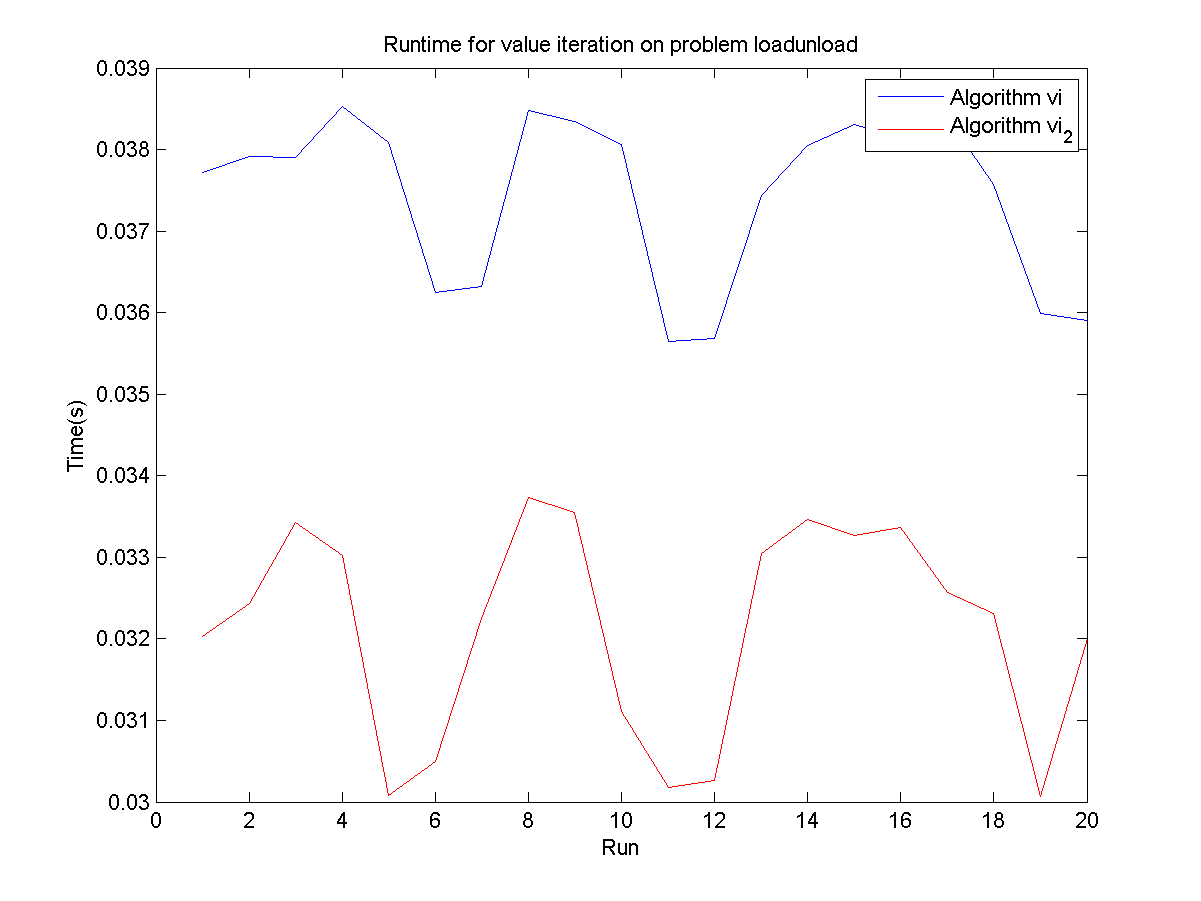
\includegraphics[width=0.7\textwidth]{Timings/loadunload/timings_vi.png}
\hspace{-30pt}
\caption{The loadunload problem}
\label{fig:vi_loadunload}
\vspace{-20pt}
\end{SCfigure}

\begin{SCfigure}
\vspace{-20pt}
\hspace{-30pt}
\centering
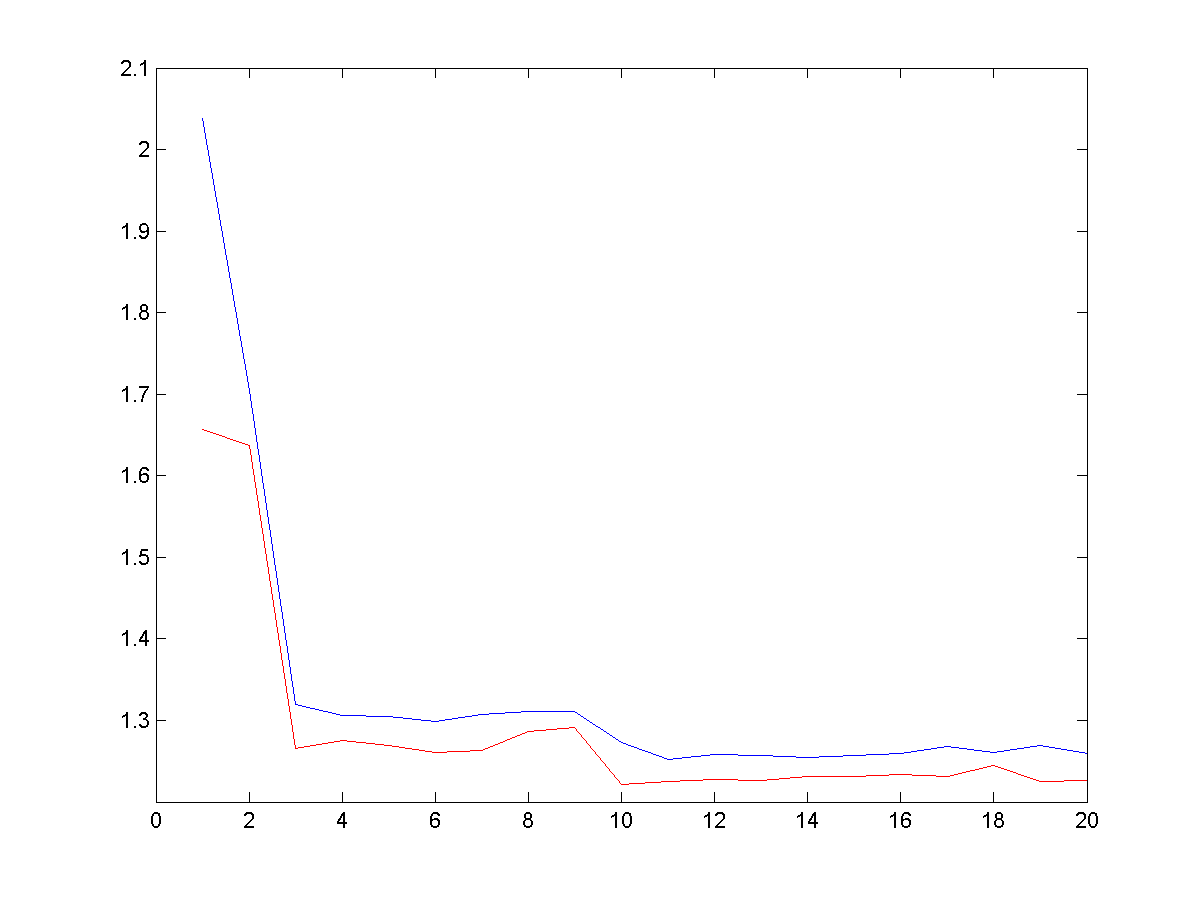
\includegraphics[width=0.7\textwidth]{Timings/hallway/timings_vi.png}
\caption{The hallway problem}
\hspace{-30pt}
\label{fig:vi_hallway}
\vspace{-20pt}
\end{SCfigure}
        
\begin{SCfigure}
\vspace{-20pt}
\hspace{-30pt}
\centering
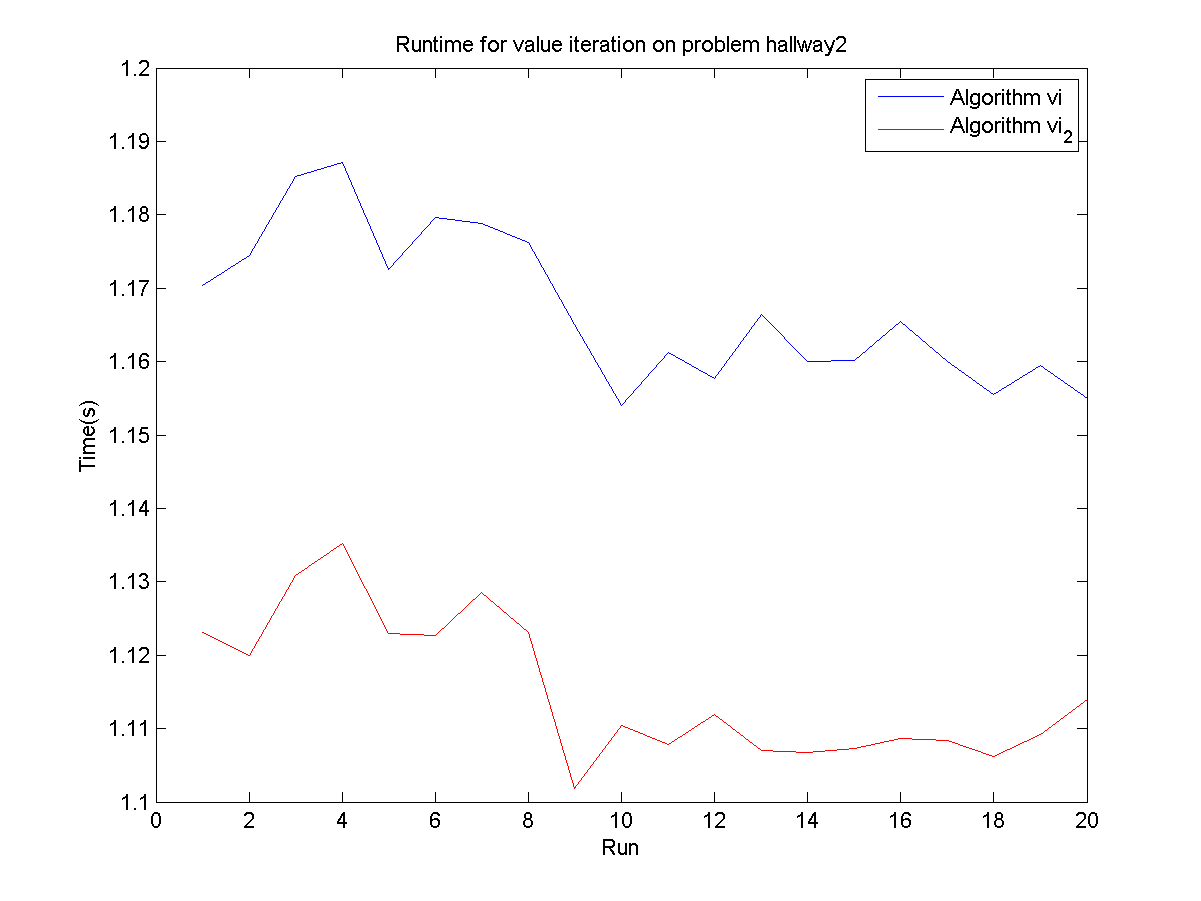
\includegraphics[width=0.7\textwidth]{Timings/hallway2/timings_vi.png}
\caption{The hallway2 problem}
\hspace{-30pt}
\label{fig:vi_hallway2}
\vspace{-20pt}
\end{SCfigure}
        
\begin{SCfigure}
\vspace{-20pt}
\hspace{-30pt}
\centering
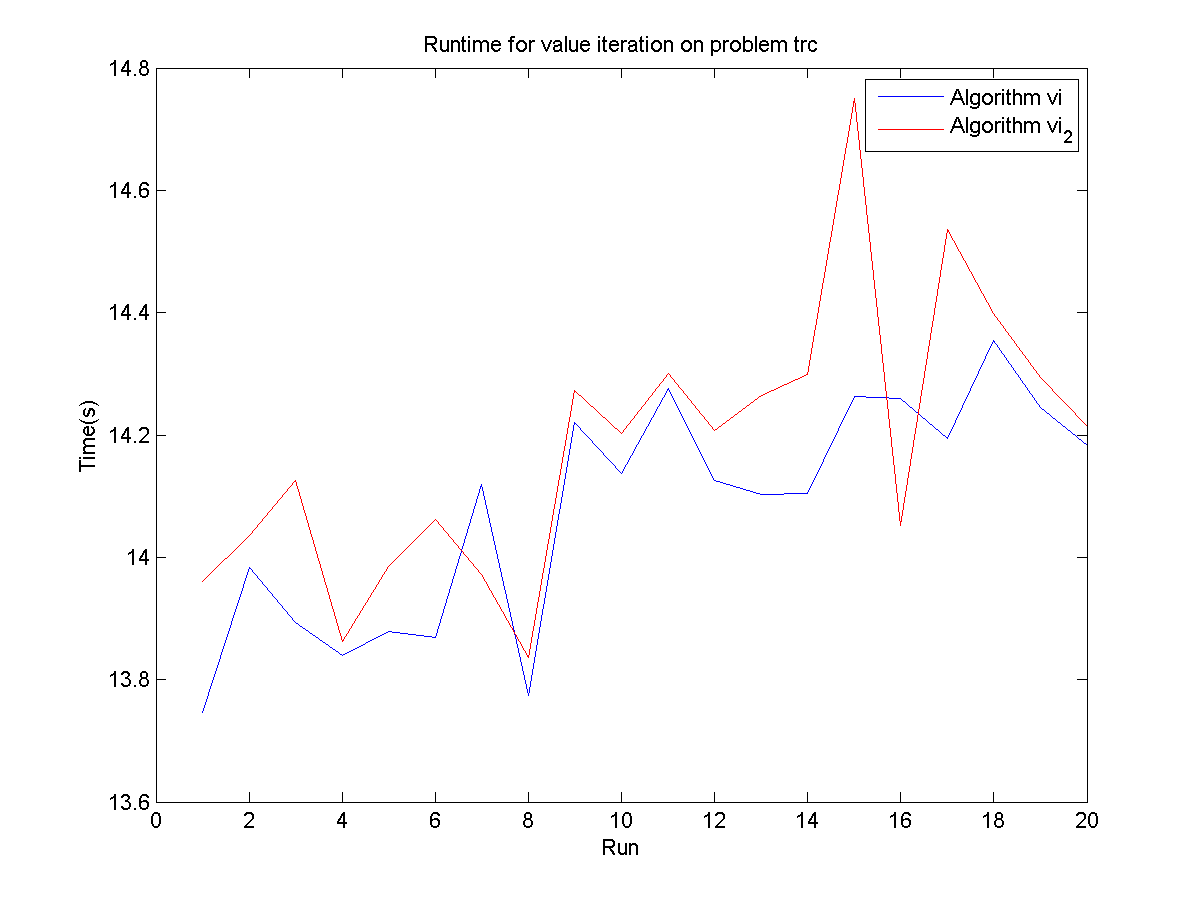
\includegraphics[width=0.7\textwidth]{Timings/trc/timings_vi.png}
\hspace{-30pt}
\caption{The trc problem}
\label{fig:vi_trc}
\vspace{-20pt}
\end{SCfigure}

%%%%%%%%%%%%%%%%%%%%%%%%%%%%%%%%%%%%%%%%%%%%%
%											%
%					Paths					%
%											%
%%%%%%%%%%%%%%%%%%%%%%%%%%%%%%%%%%%%%%%%%%%%%

\subsubsection*{Paths followed}

In figures \ref{fig:path_hallway} and \ref{fig:path_trc} a path followed in the hallway and trc problem is visualized.
This is done by first displaying the respective state and using the height of the bars or darkness of the circles to show the continuation in time. 
If a state is visited multiple times the last visit is drawn.

The figures marked (b) show which states are visited throughout the run itself.

\newgeometry{textwidth=16cm}
\begin{figure}
        \centering
        \begin{subfigure}{0.48\textwidth}
                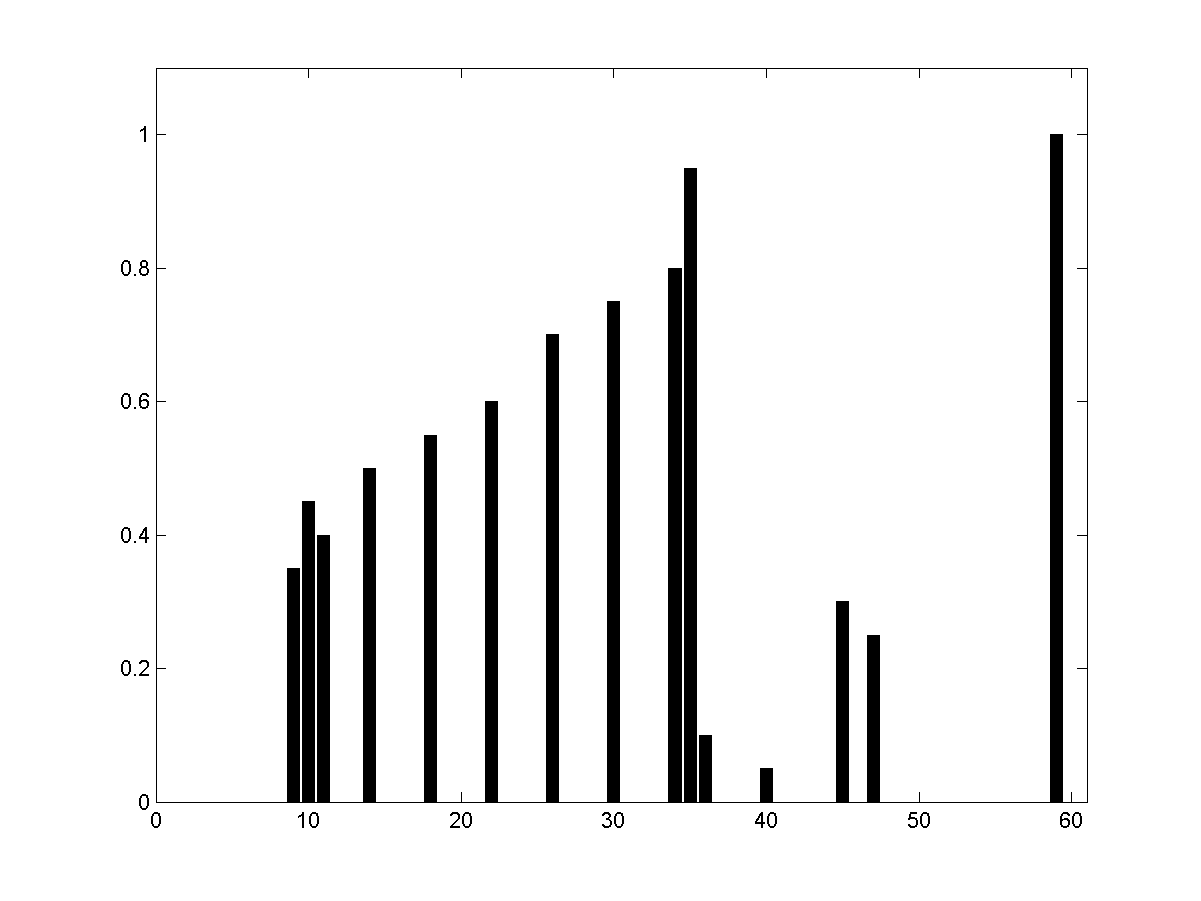
\includegraphics[width=\textwidth]{Paths/hallway/plot-basic-part1-4096896640.png}
                \caption{Last time in state, higher means more recent}
                \label{fig:path_hallway_part1}
                \hspace{10pt}
        \end{subfigure}
        \quad
        \begin{subfigure}{0.48\textwidth}
        		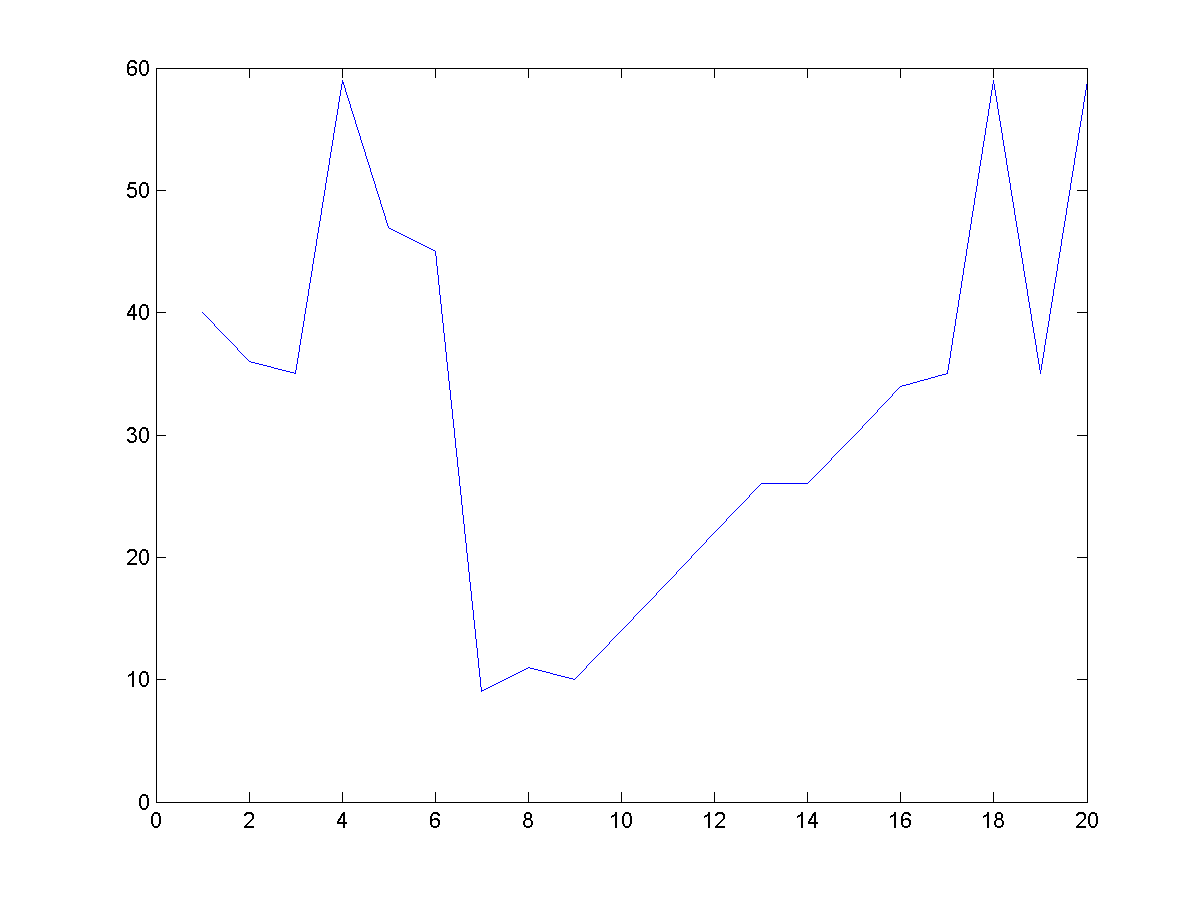
\includegraphics[width=\textwidth]{Paths/hallway/plot-basic-part2-4096896640.png}
                \caption{Run through the states}
                \label{fig:path_hallway_part2}
                \hspace{-10pt}
        \end{subfigure}
        \caption{A path through the hallway problem}
        \label{fig:path_hallway}
\end{figure}

\begin{figure}
        \centering
        \begin{subfigure}{0.48\textwidth}
        		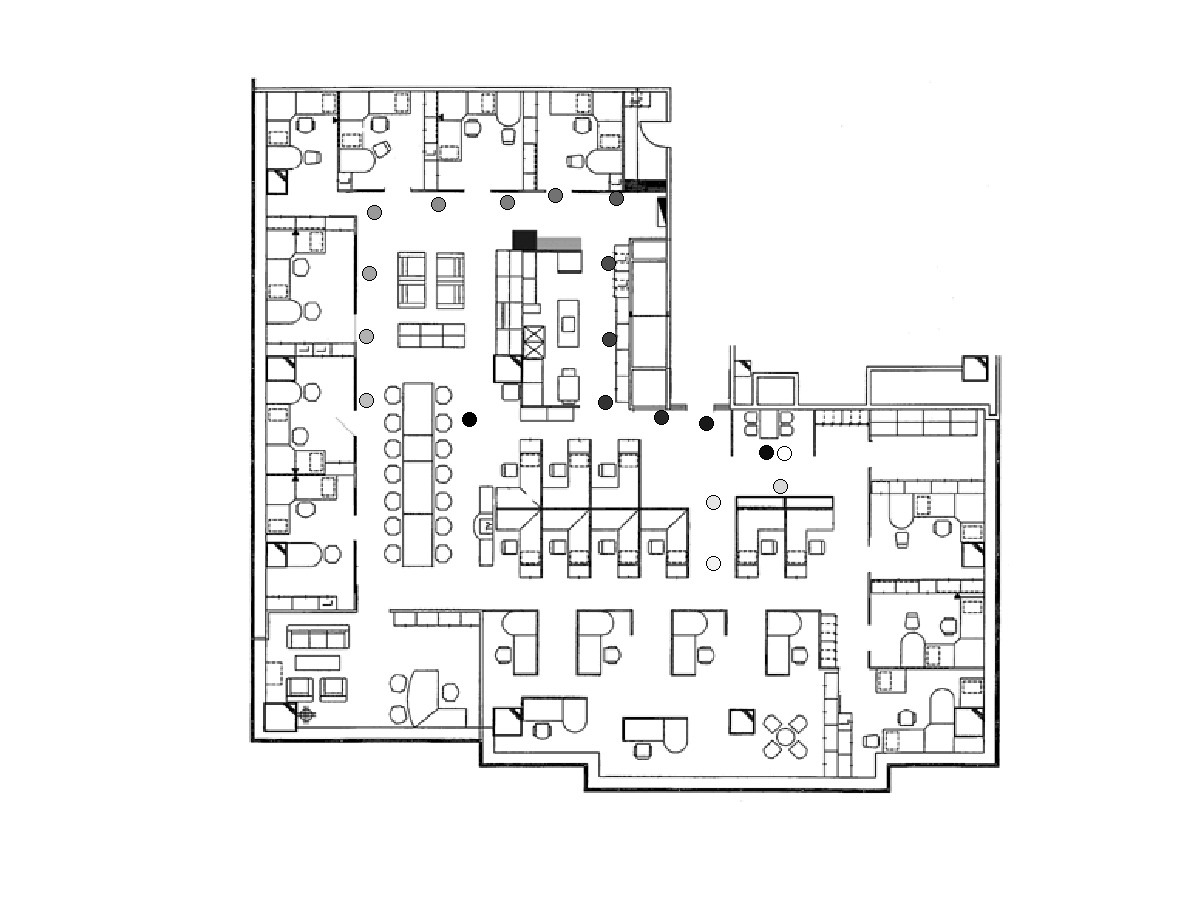
\includegraphics[width=\textwidth]{Paths/trc/plot-basic-part1-6129604379.png}
                \caption{Last time in state, higher means more recent}
                \label{fig:path_trc_part1}
                \hspace{10pt}
        \end{subfigure}
        \quad
        \begin{subfigure}{0.48\textwidth}
        		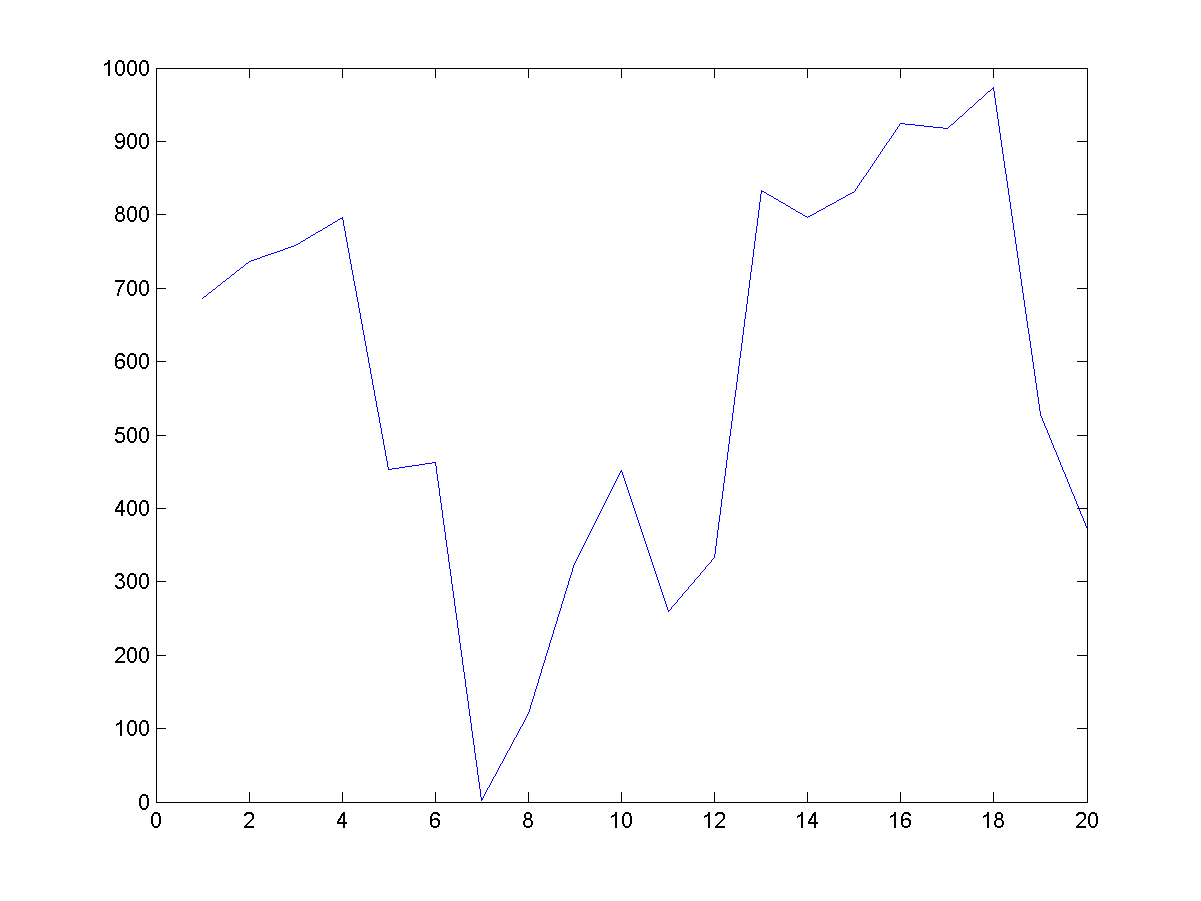
\includegraphics[width=\textwidth]{Paths/trc/plot-basic-part2-6129604379.png}
                \caption{Run through the states}
                \label{fig:path_trc_part2}
                \hspace{-10pt}
        \end{subfigure}
        \caption{A path through the trc problem}
        \label{fig:path_trc}
\end{figure}

\restoregeometry

%%%%%%%%%%%%%%%%%%%%%%%%%%%%%%%%%%%%%%%%%%%%%
%											%
%				Heuristic					%
%											%
%%%%%%%%%%%%%%%%%%%%%%%%%%%%%%%%%%%%%%%%%%%%%

\section{Partially observable environments: heuristic methods}

In table \ref{table:rewards} a comparison between the different algorithms can be seen, with averages and standard deviation over 100 runs, each with a horizon of 100 steps.
While the fully observable case produces high reward values with a relatively small standard deviation, the MLS and $Q_{MDP}$ implementations output lower and much more varied results.

The $Q_{MDP}$ implementation often stalls during execution when a state is reached where staying in the current state is the best available action.
An extreme example here is the result achieved (or clear lack thereof) with the trc problem, where not a single run produced a reward. \todo{figuur}

An explanation for this behaviour is the fact that operation in a partially observable environment lacks total information and thus can't always calculate the best possible course of actions.

%%%%%%%%%%%%%%%%%%%%%%%%%%%%%%%%%%%%%%%%%%%%%
%											%
%				Point-based					%
%											%
%%%%%%%%%%%%%%%%%%%%%%%%%%%%%%%%%%%%%%%%%%%%%

\section{Partially observable environments: point-based methods}

%%%%%%%%%%%%%%%%%%%%%%%%%%%%%%%%%%%%%%%%%%%%%
%											%
%					Part II					%
%											%
%%%%%%%%%%%%%%%%%%%%%%%%%%%%%%%%%%%%%%%%%%%%%

\part{}

%%%%%%%%%%%%%%%%%%%%%%%%%%%%%%%%%%%%%%%%%%%%%
%											%
%				Multi-agent					%
%											%
%%%%%%%%%%%%%%%%%%%%%%%%%%%%%%%%%%%%%%%%%%%%%

\section{Multiagent planning under uncertainty}

%%%%%%%%%%%%%%%%%%%%%%%%%%%%%%%%%%%%%%%%%%%%%
%											%
%				Final Remarks				%
%											%
%%%%%%%%%%%%%%%%%%%%%%%%%%%%%%%%%%%%%%%%%%%%%

\part{Final remarks}

%%%%%%%%%%%%%%%%%%%%%%%%%%%%%%%%%%%%%%%%%%%%%
%											%
%			Overview of Algorithms			%
%											%
%%%%%%%%%%%%%%%%%%%%%%%%%%%%%%%%%%%%%%%%%%%%%

\section{Overview of Algorithms}

%%%%%%%%%%%%%%%%%%%%%%%%%%%%%%%%%%%%%%%%%%%%%
%											%
%				Time Spent					%
%											%
%%%%%%%%%%%%%%%%%%%%%%%%%%%%%%%%%%%%%%%%%%%%%

\section{Time Spent}



\end{document}
